%%%%%%%%%%%%%%%%%%%%%%%%%
%% Template for small reports
%%%%%%%%%%%%%%%%%%%%%%%%%

\documentclass[letterpaper,notitlepage,10pt]{article}

%Additional packages
\usepackage{fullpage} %For using small margins 
\usepackage{latexsym}
\usepackage{amssymb}
\usepackage{amsmath}
\usepackage[english]{babel}
\usepackage[pdftex]{color,graphicx} %Images for pdfs
\usepackage[pdftex,colorlinks]{hyperref} %Hyperlinked pdfs
\usepackage{listings} %For adding code

%If you need to add math
\newenvironment{proof}{\begin{trivlist} \item[] {\em Proof:}}{\hfill $\Box$ \end{trivlist}}
\newtheorem{theorem}     {Theorem}
\newtheorem{lemma}       {Lema}
\newtheorem{observation} {Observation}
\newtheorem{proposition} {Proposition}
\newtheorem{conjecture}  {Conjecture}
\newtheorem{corollary}   {Corolari}
\newtheorem{property}    {Property}
\newtheorem{definition}  {Definition}

%Title box
\newcommand{\titlebox}[6]
{\noindent\fbox{\parbox{\textwidth}{#1 \hfill\textbf{#2}\begin{center} 
\LARGE #3 \end{center}#4 $<$\href{mailto:#5}{#5}$>$ \hfill #6}}\bigskip\\}

%If you want to include code
%standard configuration of the listings package
%\lstset{language=matlab, basicstyle=\footnotesize, numbers=left, frame=lines, frameround=tfft,breaklines=true}
%how to include a file "\lstinputlisting{../../Courses/16720-CV/hw2/matlab/blockify.m}"


%%%%%%%%%%%%%%%%%%%%%%
%% Here begins the document
%%%%%%%%%%%%%%%%%%%%%%
\begin{document}
\titlebox
{CMU  - Robotics Institute} % Institution (ex: CMU - Robotics Institute)
{Manipulation Lab}              % Center (ex: Manipulation Lab)
{ABB Robot I/O (IRC5 controller)}                                  % Title
{Alberto Rodriguez}             % Author
{albertor@cmu.edu}           % e-mail
{2010/12/03}                      % Date (format yyyy/mm/dd)

This is a brief tutorial on how I/O works on IRC5 ABB controller and
how to set up input and output signals.

\section{Physical level}
The ABB controller supports communication boards: Ethernet, DeviceNet,
PROFIBUS and INTERBUS. They are located in the vertical racks in a PC
inside the controller, Fig.~\ref{fig:PC}.
%
\begin{figure}[h]
	\centering
		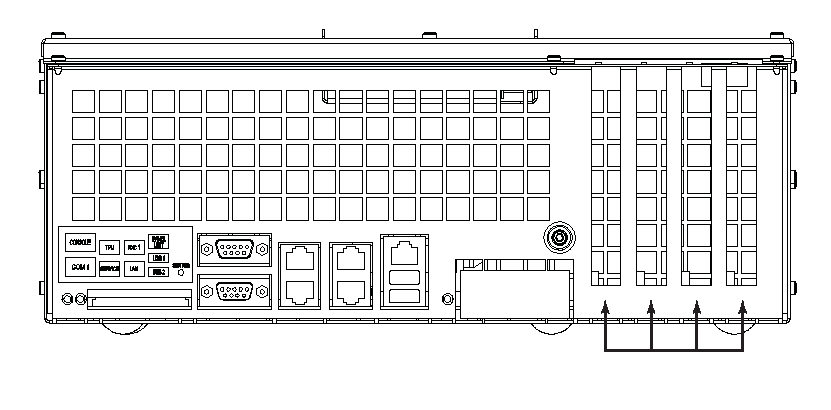
\includegraphics[width=4in]{figures/PC}
                \caption{PC internal to the ABB controller.}
	\label{fig:PC}
\end{figure}
%
The controller in the Manipulation Lab has a DeviceNet board installed
in the leftmost vertical rack. 

DeviceNet communication consists of a Master/Slave structure. The
board in the vertical rack (DSQC 658) is the master and distributed or
slave I/O units connect to it, including units with digital I/O (DSQC
652), analog I/O (DSQC 355A), digital I/O with relays (DSQC 653) or
various combinations.  The controller in the Manipulation Lab has a
DSQC 652 slave I/O unit, Fig.~\ref{fig:DSQC652}, located in the back
of the front door. It allows for 16 digital outputs and 16 digital
inputs, all working with 24 V logic.
%
\begin{figure}[h]
	\centering
		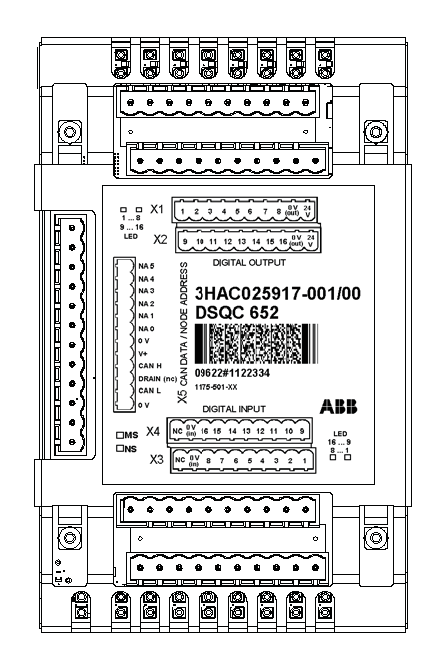
\includegraphics[width=2in]{figures/DSQC652}
                \caption{DSQC 652 I/O unit in the back of the front
                  door of the IRC5 controller.}
	\label{fig:DSQC652}
\end{figure}
%
The top connectors are optically isolated digital outputs and the
bottom ones are optically isolated digital inputs. The unit is
correctly setup and working if the two LEDS (NS and MS) in the bottom
right corner are green.
\\

To physically connect a digital output you have to:
\begin{itemize}
\item Supply 24V power source to pin 10 of X1 connector.
\item Connect ground power source to pin 9 of X1 connector.
\item Draw output signal from the correspondent pin in X1 or X2
  connector. Output channels 1 to 8 are mapped to pins 1 to 8 in
  X1. Output channels 9 to 16 are mapped to pins 1 to 8 in connector
  X2.
\end{itemize}

A more detailed description of the connectors and LEDs in the DSQC 652
I/O unit can be found on pages 77-81 of the Application Manual:
DeviceNet.

\section{Software level}

Three things need to be configured at software level to use the I/Os
of the controller:
\begin{itemize}
\item Communication Bus (Device Net).
\item I/O Unit connected to the bus (DSQC 652).
\item Input and output signals mapped to the I/O unit.
\end{itemize}

\subsection{Bus}
A bus is an abstraction of a communication device.  It is configured
inside I/O system parameters --- through the teach pendant: Control
Panel $\rightarrow$ Configuration $\rightarrow$ I/O Topic
$\rightarrow$ Bus.  Inside Bus, there should be a DeviceNet bus
configured.  In the case of the Manipulation Lab controller, it is
named DeviceNet1.
\\

Configuration parameters:
\begin{description}
\item \textbf{Type} DeviceNet.
\item \textbf{Master Address} 2 in the case of the Mlab controller.
\item \textbf{Communication Speed} 500kbs in the case of the Mlab
  controller.
\end{description}
For a detailed description of the rest of parameters, look into pages
138-146 of the Technical Reference Manual: System Parameters.

\subsection{Unit}
A unit is an abstraction of a slave device connected to a bus.  It is
configured inside I/O system parameters --- through the teach pendant:
Control Panel $\rightarrow$ Configuration $\rightarrow$ I/O
Topic $\rightarrow$ Unit.  Inside Unit there should
be a device that represents the unit connected to the DeviceNet
bus. In the case of the Manipulation Lab controller, it has the name IOboard and
represents the DSQC 652 unit in the back of the front door.
\\

Configuration parameters:
\begin{description}
\item \textbf{Name} User defined name of the slave I/O unit (IOboard).
\item \textbf{Type of Unit} Identifies the type of slave I/O unit
  connected to the Bus (d652).
\item \textbf{Connected to Bus} Bus where the slave I/O unit is
  connected (DeviceNet1).
\item \textbf{Unit Identification Label} User defined description of
  the unit.
\item \textbf{DeviceNetAddress} Number 0-63 that identifies the
  address of the slave I/O unit in the bus.
  
  The address is coded in binary in the pins 7-12 of the X5 connector
  in the same slave unit.  Fig.~\ref{fig:busID} shows the binary
  codification of the address with the pins. The configuration in the
  figure is the one present in the Manipulation Lab controller,
  yielding address 10.
%
\begin{figure}[h]
	\centering
		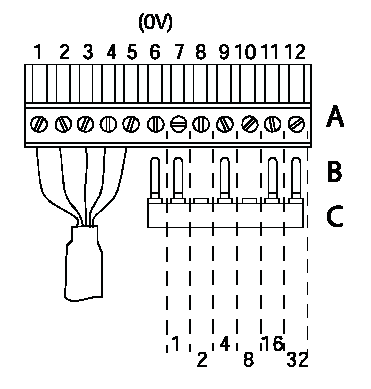
\includegraphics[width=2.5in]{figures/busID}
                \caption{Configuration of the DeviceNet bus
                  ID. Example: cut address pins 8 and 10 to obtain
                  address 10.}
	\label{fig:busID}
\end{figure}
%
\end{description}

\subsection{I/O Signals}
To create a new I/O signal, go to Control Panel $\rightarrow$
Configuration $\rightarrow$ IO/Topic $\rightarrow$ Signal
$\rightarrow$ Add.
\\

Configuration Parameters:
\begin{description}
\item \textbf{Name} Name to use to access the signal through RAPID.
\item \textbf{Type of signal} To choose from: Digital Input, Digital
  Output, Analog Input, Analog Output, Group Input and Group
  Output. In the case of the Mlab controller, only digital signals are
  available.
\item \textbf{Assigned to Unit} Unit where the signal will be assigned
  to (IOboard).
\item \textbf{Signal Identification Label} User defined description of
  the signal.
\item \textbf{Unit Mapping} Number identifying the input/output pin in
  the I/O unit. The numbers 0-15 map to the channels 1-16, as shown in
  Fig.~\ref{fig:mapping}.
%
\begin{figure}[h]
	\centering
		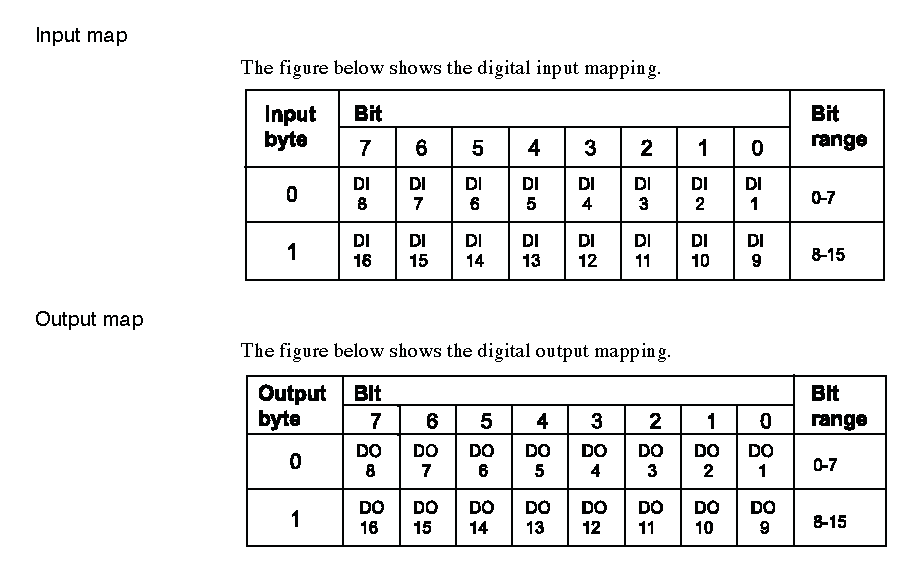
\includegraphics[width=5in]{figures/mapping}
                \caption{Digital input and output mapping.}
	\label{fig:mapping}
\end{figure}
%
\end{description}


%%%%%%%%%%%%%%%%%%%%
%% If you want bibliography
%%%%%%%%%%%%%%%%%%%%
%\bibliographystyle{unsrt}
%\bibliography{} %Name and location of the bibfile

%To cite a reference -> \cite{cite_name}
%To make a reference appear in the bibliography without a citation in the text -> \nocite{cite_name}

\end{document}
